% Metódy inžinierskej práce

\documentclass[10pt,twocolumn,twoside,slovak,a4paper]{article}

\usepackage[slovak]{babel}
\usepackage[IL2]{fontenc} % lepšia sadzba písmena Ľ než v T1
\usepackage[utf8]{inputenc}
\usepackage{graphicx} % na vkladanie obrázkov
\usepackage{url} % príkaz \url na formátovanie URL
\usepackage{hyperref} % odkazy v texte budú aktívne (pri niektorých triedach dokumentov spôsobuje posun textu)
\usepackage{cite} % na správne citovanie
\usepackage{subcaption} % na vedľajšie obrázky
\usepackage{wrapfig} % na plávajúce obrázky

\pagestyle{headings}

\begin{wrapfigure}{r}{0.25\textwidth}
  \centering
  \includegraphics[width=0.2\textwidth]{fiit_logo.png}
\end{wrapfigure}


\title{Názov\thanks{Semestrálny projekt v predmete Metódy inžinierskej práce, ak. rok 2024/25, vedenie: Richard Marko}} % meno a priezvisko vyučujúceho na cvičeniach

\author{Roman Dunko\\[2pt]
	{\small Slovenská technická univerzita v Bratislave}\\
	{\small Fakulta informatiky a informačných technológií}\\
	{\small \texttt{xdunko@stuba.sk}}
}

\date{\small 10. október 2024}

\begin{document}

\maketitle

\begin{abstract}
\ldots
\end{abstract}

\section{Úvod}
Vplyv odporúčacích systémov na personalizované nakupovanie v elektronickom obchode

Odporúčacie systémy sú dnes neodmysliteľnou súčasťou elektronického obchodu. Je ťažké nájsť obchod, ktorý nevyužíva tieto výdobytky doby. Tieto systémy využívajú algoritmy na analýzu správania zákazníkov a vytvárajú personalizované odporúčania produktov, ktoré zvyšujú šance na dokončenie nákupu. Mojím cieľom je skúmať, ako tieto systémy ovplyvňujú nákupné správanie spotrebiteľov, a to z pohľadu rozhodovacieho procesu aj celkového zážitku z nakupovania.

Základný problém, ktorý bol naznačený v úvode, je podrobnejšie vysvetlený v časti~\ref{nejaka}.
Dôležité súvislosti sú uvedené v častiach~\ref{dolezita} a~\ref{dolezitejsia}.
Záverečné poznámky prináša časť~\ref{zaver}.

\section{Nejaká časť} \label{nejaka}

Z obr.~\ref{f:rozhod} je všetko jasné. 

\begin{figure*}[tbh]
\centering
\caption{Rozhodujúci argument.}
\label{f:rozhod}
\end{figure*}

\section{Dva obrázky vedľa seba}

\begin{figure*}[h!]
\centering
\begin{subfigure}{.45\textwidth}
  \centering
  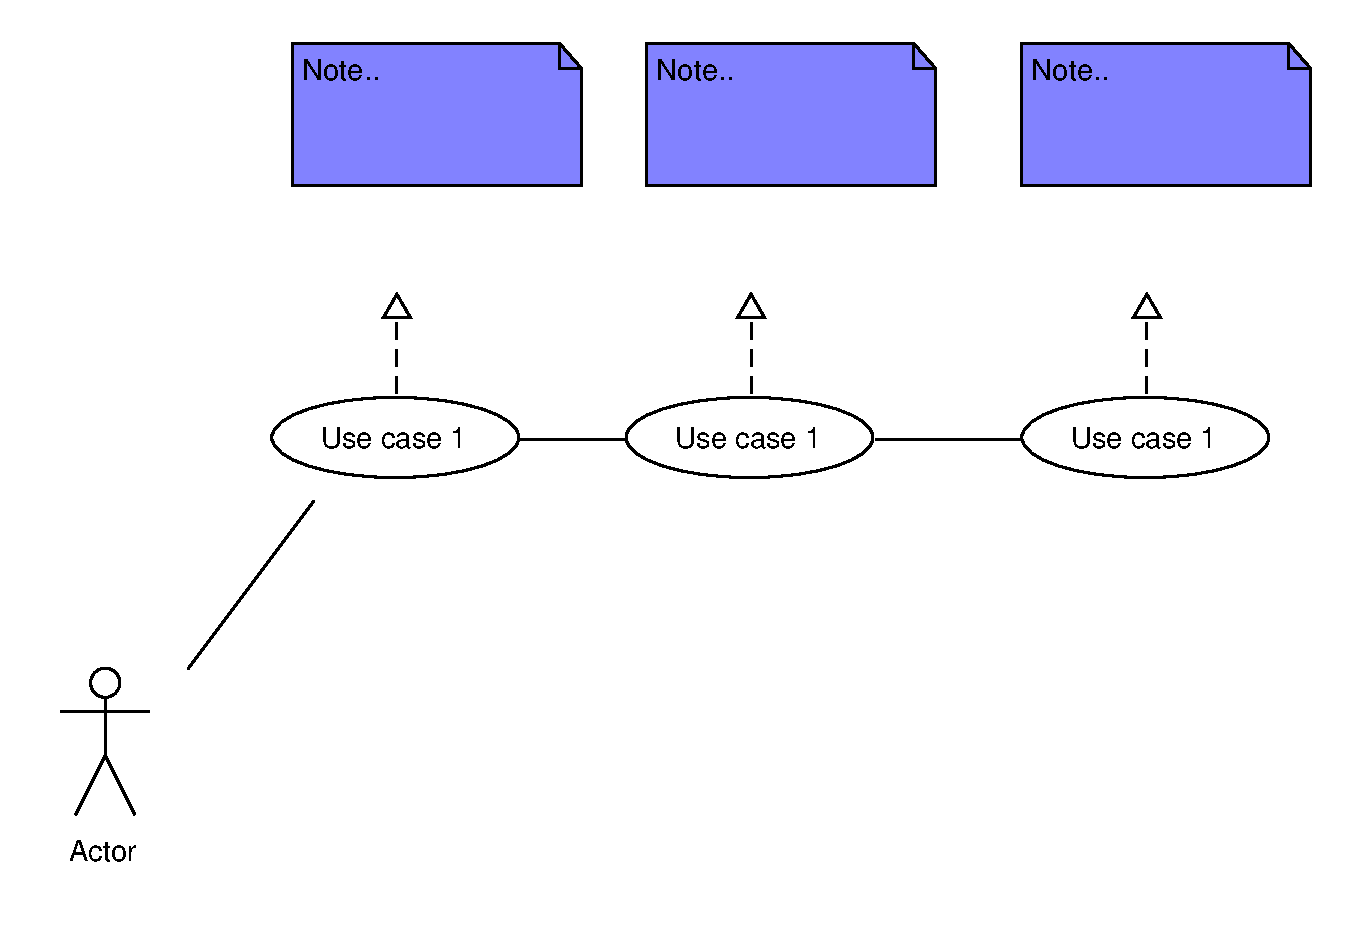
\includegraphics[width=\linewidth]{graf1.pdf} % Prvý graf
  \caption{Graf 1}
\end{subfigure}%
\hfill
\begin{subfigure}{.45\textwidth}
  \centering
  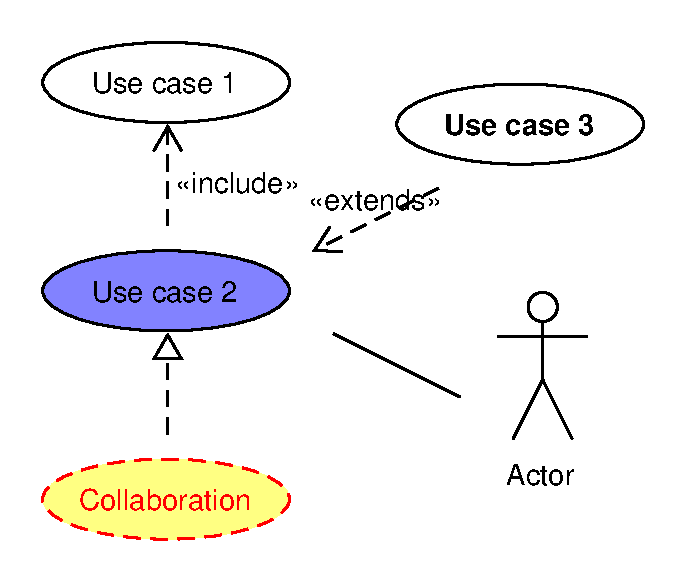
\includegraphics[width=\linewidth]{graf2.pdf} % Druhý graf
  \caption{Graf 2}
\end{subfigure}
\caption{Dva grafy vedľa seba}
\end{figure*}

\section{Dôležitá časť} \label{dolezita}
Dôležitý obsah článku.

\section{Ešte dôležitejšia časť} \label{dolezitejsia}
Ešte dôležitejší obsah článku.

\section{Záver} \label{zaver}
Záver článku.

\bibliography{literatura} % odkaz na súbor literatura.bib
\bibliographystyle{plain} % štýl bibliografie

\end{document}
